\chapter{Proposed Solution}
\label{chap:proposed-Solution}

Our initial motivation for this thesis was to enable visualization of hierarchical and disjoint grouped datasets in VR. 
Data scientists often deal with these datasets and because of the complexity of the data they often have to rely on classical 2D visualization software.
However, current 2D approaches quickly reach their limits and run into the problem of visual clutter, especially when visualizing large networks and deep hierarchies. For example the comorbidity network shown in Figure \ref{fig:2dHierarchicalClutter} hides links and is limited to only one hierarchical layer. Instead of limiting ourselves to one hierarchical layer, we wanted a solution to visualize any number of hierarchical layers.
To improve the process of hierarchical network exploration, we wanted to use the capabilities of VR and 3D information visualization. In Section \ref{sec:motivation}, we summarized how these techniques can be beneficial for network visualizations.  

\section{Requirements}
\label{chap:ps-requirements}
We defined multiple requirements based on the problems we described in the previous chapters:\\
\begin{enumerate}
    \item[R1]\label{req:R1} The visualization is able to visualize a hierarchical and disjoint network with depth $n$. Each node can be a super-node or meta-node. Links are possible within nodes of the same parent super-node but also to nodes of different super-nodes with the same hierarchical depth.
    \item[R2]\label{req:R2} The visualization can display larger networks than classical 2D approaches, before reaching a critical point of visual clutter where a meaningful exploration is not possible anymore.
    \item[R3]\label{req:R3} The visualization supports a seated, standing and room scale experience for small and large room sizes.
    \item[R4]\label{req:R4} The visualization fully utilizes the tracking capabilities of the VR Headset to optimize the interaction experience for the user.
    \item[R5]\label{req:R5} The visualization allows a flexible navigation through the graph during the exploration process.
    \item[R6]\label{req:R6} The visualization ensures a clear overview of the entire data by applying appropriated techniques according to Shneiderman's visualization seeking mantra.
    \item[R7]\label{req:R7} The visualization ensures that deep hierarchical networks can be explored using familiar interaction techniques and reduces the problem of a multi scale scene.
    \item[R8]\label{req:R8} The visualization uses the HTC Vive as a target platform, but the concepts should be transferable to other 6-DOF Headsets. 
\end{enumerate}

\section{Layout}
\label{chap:ps-layout}

\begin{figure}[h]
    \centering
    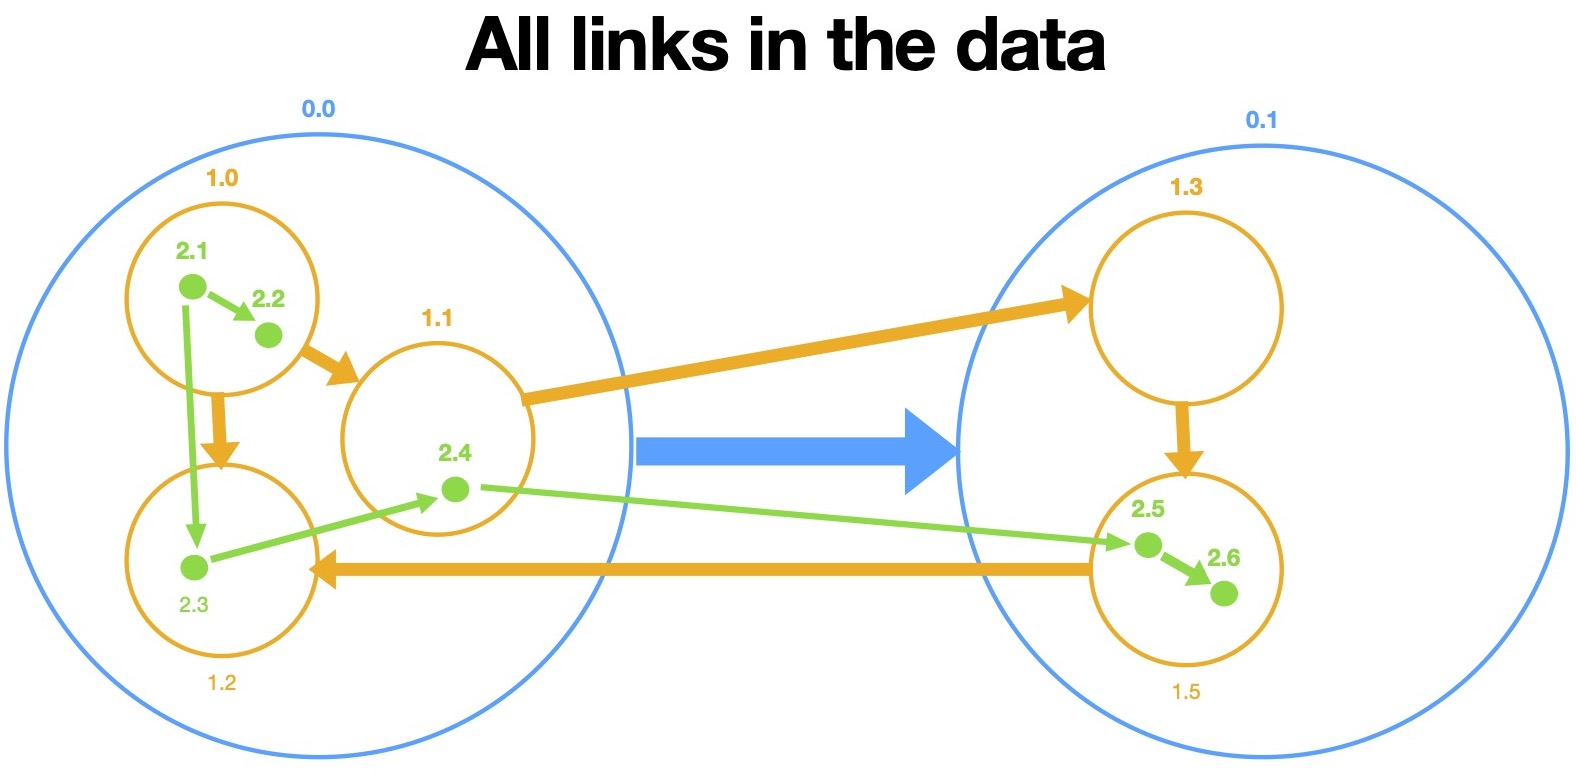
\includegraphics[width=\textwidth, trim={0cm 0cm 0cm 3.5cm},clip]{graphics/filterLinks/allLinks.jpg}
    \caption[A sketch of our layout in 2D.]{A sketch of our layout approach in 2D. Instead of 2D circles, we use 3D spheres in the real application. The size of the nodes is determined by their depth and number of child nodes. The node labels describe their unique ID. This ID consists of two parts: the first number before the dot represents the depth, respectively the layer of the node; the second part is a unique number identifying the node within one layer.} 
    \label{fig:layoutSketch} 
\end{figure}
To achieve \hyperref[req:R1]{R1}, we created a variation of circle packing layout approaches. The core concept is to combine the nested technique of tree maps with multilayer techniques. However instead of flat surfaces as seen in many multilayer network visualizations, we use three-dimensional spheres. 
By using the third dimension, we can achieve a better distribution of nodes and links and therefore display larger networks than with classical 2D approaches, as required in \hyperref[req:R2]{R2}. 
To dynamically build this layout for any given data as input, we developed a custom force based system.
The main goal is to prevent overlapping of nodes while still visualizing the different clusters of hierarchical nodes by proximity. Figure \ref{fig:layoutSketch} shows a sketch of our envisioned layout. The entire data can be seen as a tree structure where each entity in the tree is a graph itself, nested in its parent node. This means that each node can be a super-node or meta-node. Therefore, the number of nodes can grow exponentially with the number of hierarchical layers. Note that the root node is not displayed because it would just create an additional complexity in the visualization without adding any meaningful benefit.

\subsection{Layout Forces and Constraints}
\label{chap:ps-forces}
The force-based layout system consists of multiple forces and constraints to automatically calculate the positions of all nodes. We want to achieve an evenly distributed graph while still fulfilling the requirement rules for hierarchical nesting. Firstly, we define a set of force and constraint templates:
\begin{itemize}
    \item ManyBody-Force: This force is a repulsion force and causes nearby nodes to be pushed away from each other. The strength decreases with the distance of the nodes. This allows the distribution of nodes evenly among the available space.
    \item Link-Force: It is the counterpart of the ManyBody-Force and pulls nodes connected via a link closer together. Together with the ManyBody-Force, it enables us to model a distributed graph while still clustering connected nodes and minimizing the chance for a link to cross a not involved node.
    \item Collision-Force: This force is basically a reinforced version of the ManyBody-Force it prevents nodes from overlapping in the case the ManyBody- and Link-Force push nodes into each other.
    \item Spherical-Constraint: The spherical-constraint is the core concept of our layout we use for nesting nodes. It allows us to “squish” multiple nodes into a sphere for any given point and radius. The center of the sphere can vary for each simulation step. The constraint works by constantly adding a slightly randomized velocity for each node towards the center of the sphere. If the node is outside the sphere, then the velocity is increased drastically.
    \item Center-Force: This force helps us to position the entire visualization in the center of our viewpoint, however there is no strict distance or radius like the Spherical-Constraint applies.
\end{itemize}

It is important to understand that these templates are not applied equally to all nodes. Instead, we apply multiple instances of these forces with different parameters to various subsets of our graph. 
This separation allows us to prevent interference between different groups of nodes for different parents.
Firstly, we distinguish between the top hierarchical layer (from now on called layer $0$) and all other subsequent layers 1,2,3 and so on. Each node and link instance is assigned their respectively layer attribute. Layer $0$ is treated separately because these nodes have no directly assigned parent node. 
For Layer $0$, the center-force with the coordinates $(x:0,y:0,z:0)$, ManyBody-Force, Collision-Force and lastly Link-Force are applied to all nodes and links with a layer $0$ attribute. 
As for layer $1$ to layer $n$, we do not apply forces by layer but instead by parent node. For each parent, we add a Collision-Force, ManyBody-Force and Link-Force for all child nodes and links. In addition, the Spherical-Constraint is also added for all child nodes with the position of the parent node as a center. Note that the position of the parent node can change each simulation iteration, so we also update the center position for the Spherical-Constraints.
In conclusion, the total number of forces and constraints in our entire force system (including all layers) is: 
\begin{equation}
    |forces| + |constraints| \: = 4 \, + 4 \cdot |parent\_nodes|
\end{equation}

\subsection{Stability of the force system}

A big challenge for our customized force system was to equally balance all added forces so that each one performs their specific task and does not influence the effect of other forces. To achieve that, we parameterized each force with a strength parameter.
In addition, we also use the concept of an $\alpha$ target from D3-Force \cite{bostock_d3forcejs_nodate}. To put it briefly, it is an additional value, which decreases throughout the simulation. This allows the simulation to “cool down” and stop as soon as it reaches the defined $\alpha$ target value. We use the $\alpha$ target to control the number of simulation iterations. 
Besides balancing the different templates of forces, we also have to decrease the strength recursively for each layer as the nodes and their radius get smaller each layer iteration.
To further improve the stability of the layout, we add a small amount of randomness to the applied velocities and strengths. This improves the node distribution and prevents scenarios where multiple nodes receive the same forces and therefore would overlap each other.
During our optimization, we stumbled upon the problem that nodes tend to jump rapidly to a far position. This happens because we squish the nodes into the sphere of the parent while still applying the ManyBody- and Collision-Forces. Therefore, in some boundary scenarios, the only “free” position for this node is further away which results in the jumping behavior. However, it defeats the concept of successively fine-tuning the positions throughout the simulation steps. For example, nodes of layer 1-3 would be already positioned well but in the last simulation step the parent node in layer 0 would jump and therefore layer 1-3 nodes are positioned outside the parent layer 0 node again. To circumvent that problem, we do not perform the positioning of all nodes throughout the entire simulation. Instead we split up the amount of simulation steps and perform them for each layer successively (see Figure \ref{fig:SimulationSteps}): beginning with positioning the layer 0 nodes, then layer 1 nodes and so on.
Luckily, we also gain a performance benefit through that strategy. 
The reason for this is that, usually the number of nodes grows exponentially for each layer. That means, that a simulation steps for layer5 has to process more individual nodes and forces than a simulation step for layer1. By limiting the simulation steps for the larger growing layers we can reduce the total sum of position update operations.
\begin{figure}[h]
    \centering
    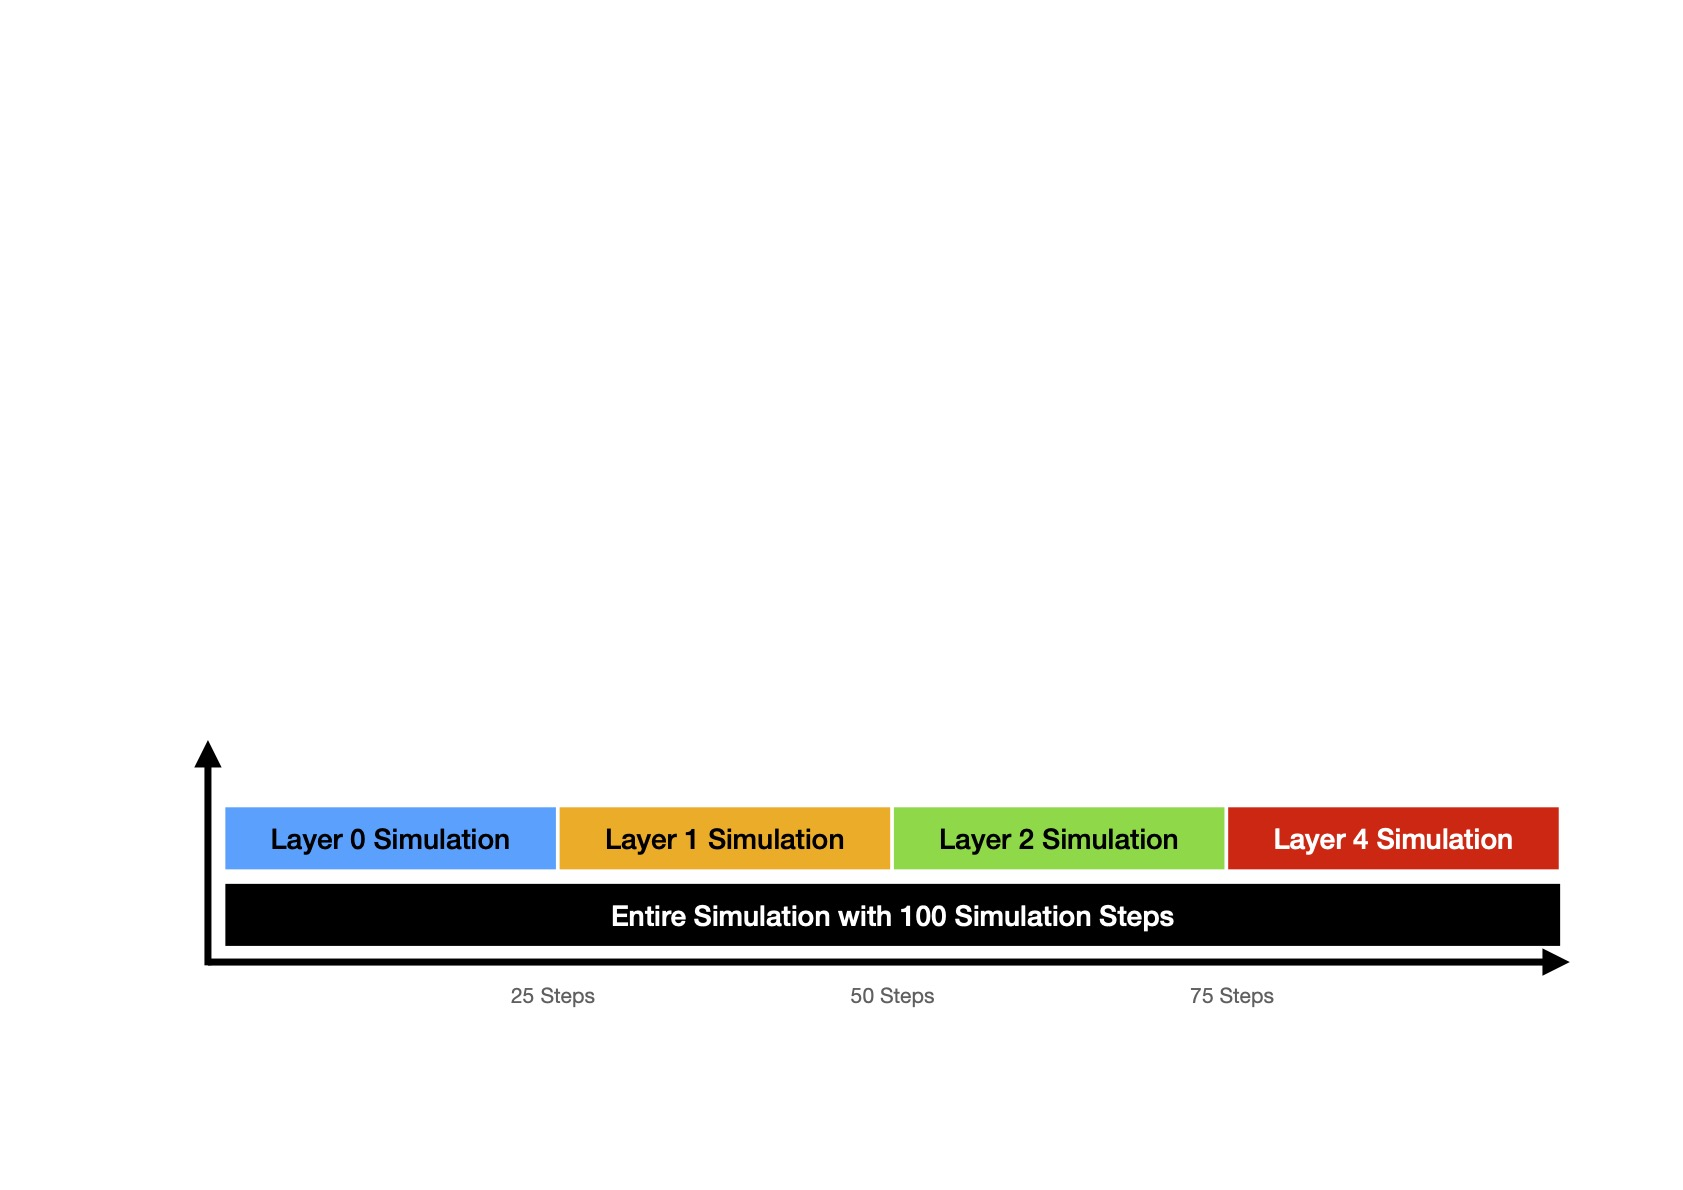
\includegraphics[width=\textwidth]{graphics/simulationStepsSplit.jpg}
    \caption[Distribution of all simulation steps.]{Distribution of all simulation steps for a dataset with 4 hierarchical layers. Each layer receives the same amount of simulation steps, in this case 25 of 100.}
    \label{fig:SimulationSteps} 
  \end{figure}

\section{Graph Visualization}
\label{chap:ps-graphRepresentation}
\begin{figure}[!htb]
    \centering
    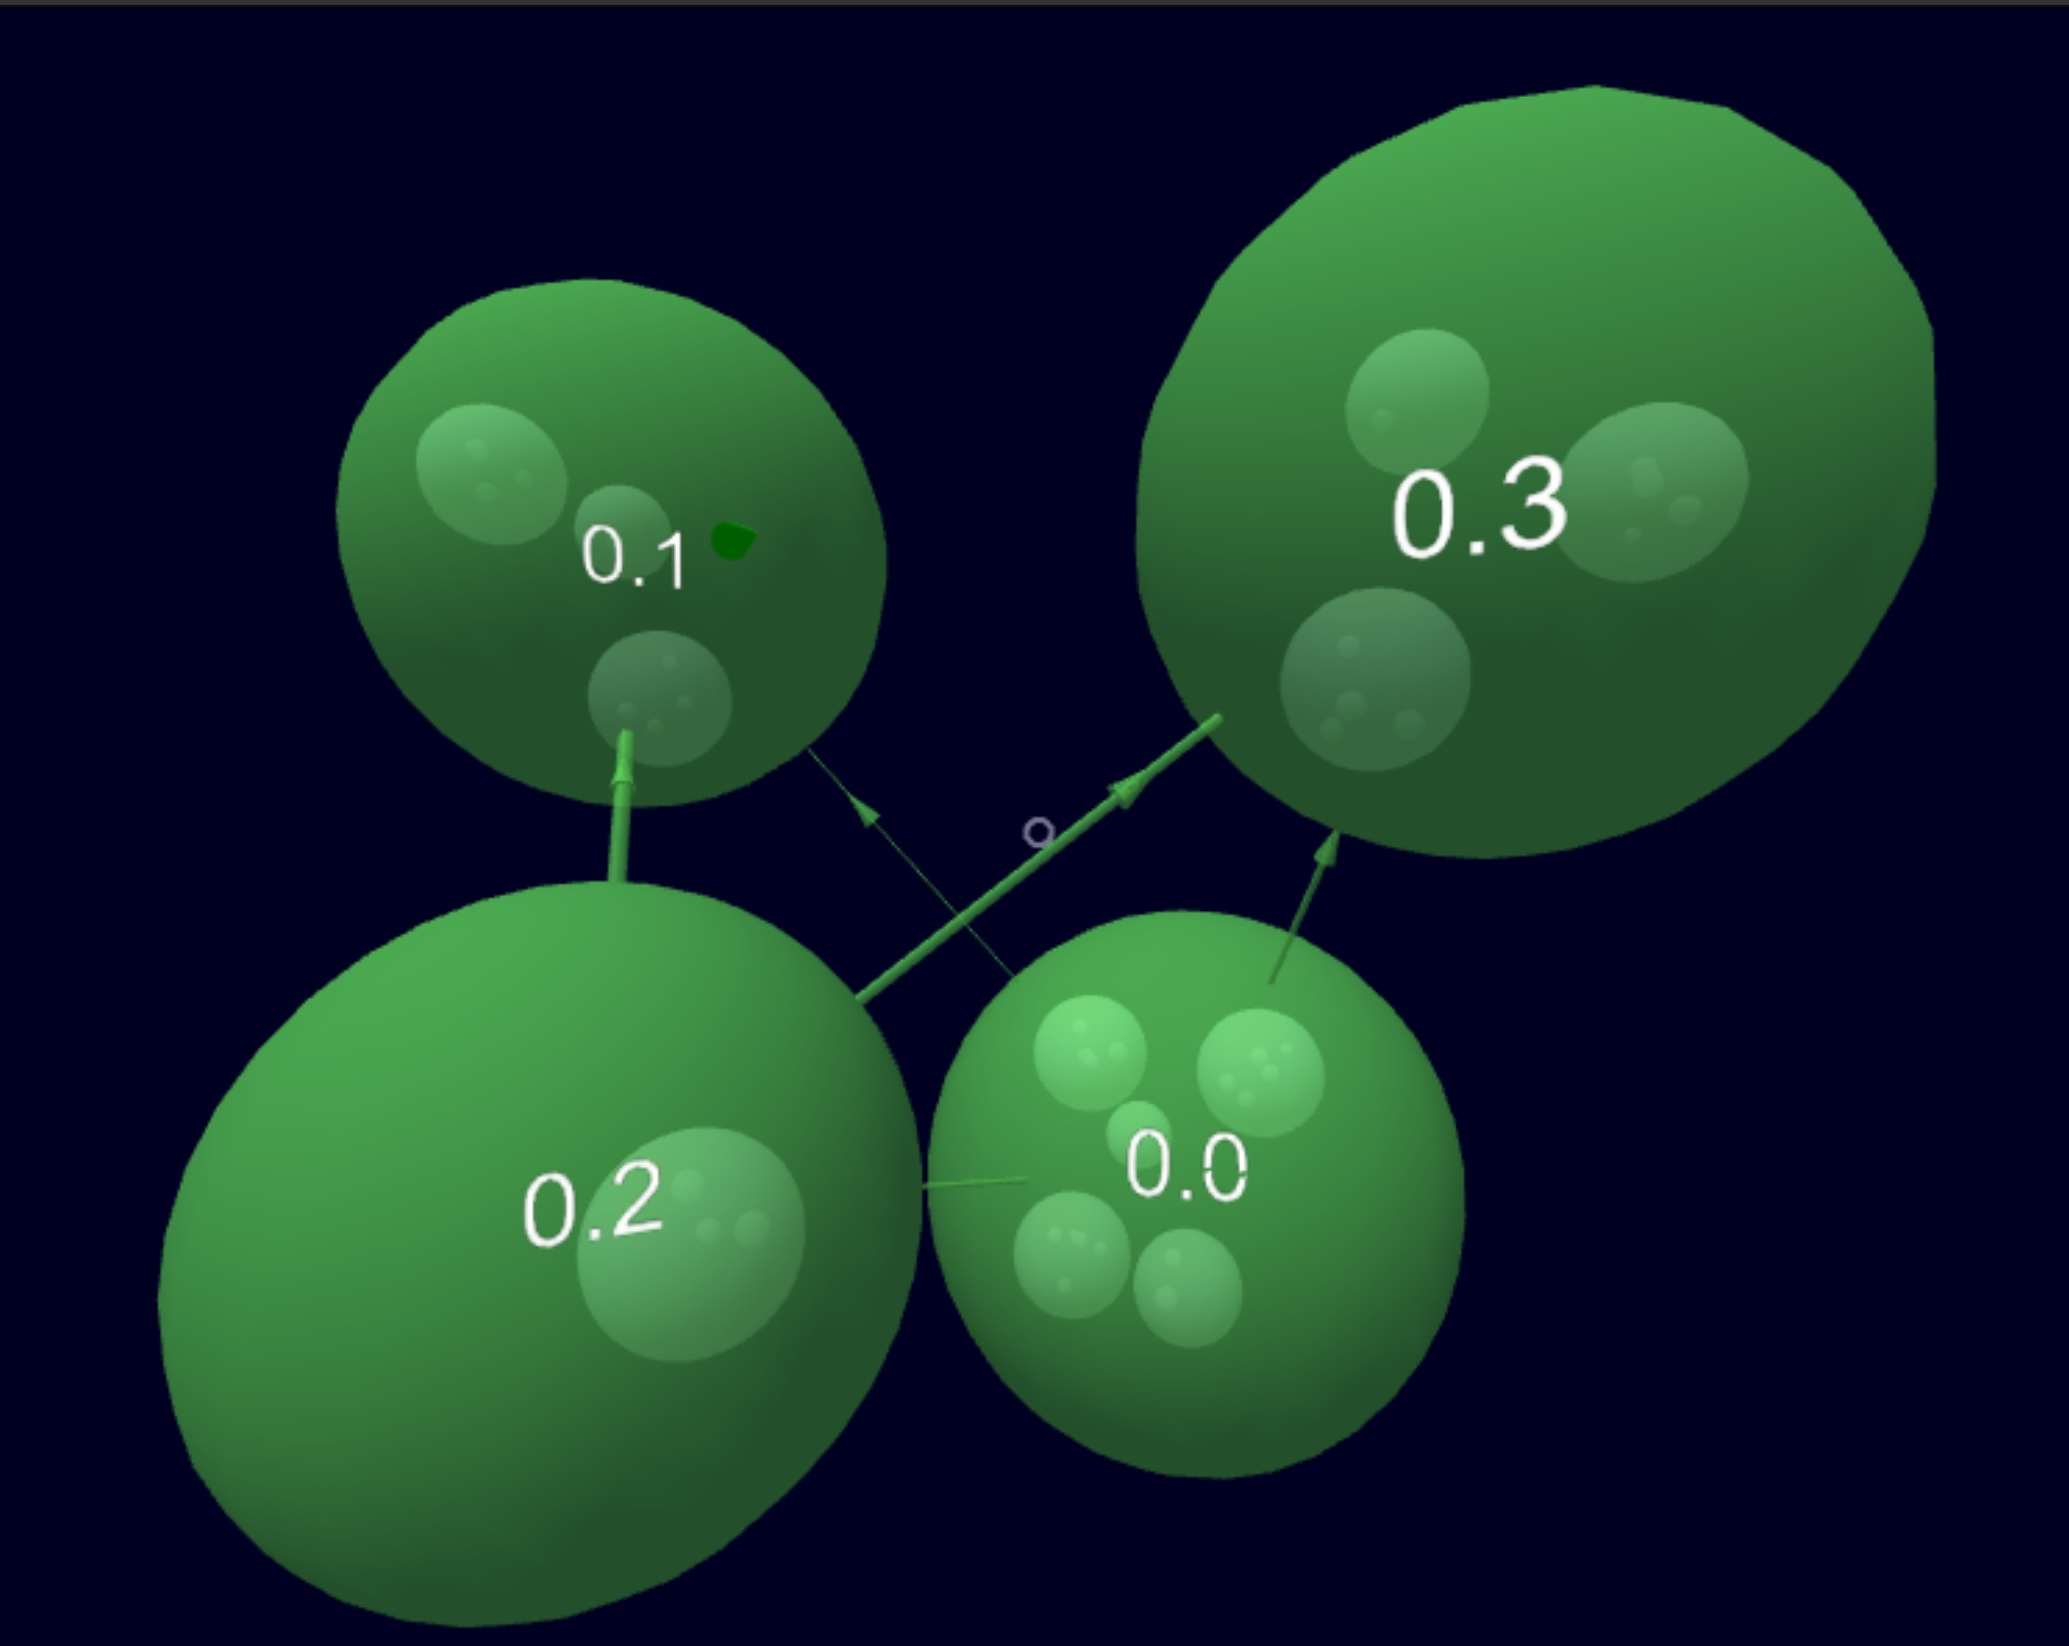
\includegraphics[width=1\textwidth]{graphics/screenshotNesting.jpg}
    \caption[Screenshot of the visualization.]{Overview perspective of the visualization: Each node is rendered semi-transparently. This allows the user to detect the overall topology of the data.}
    \label{fig:ps_nestedLayout}
\end{figure}
\begin{figure}[!htb]
    \centering
    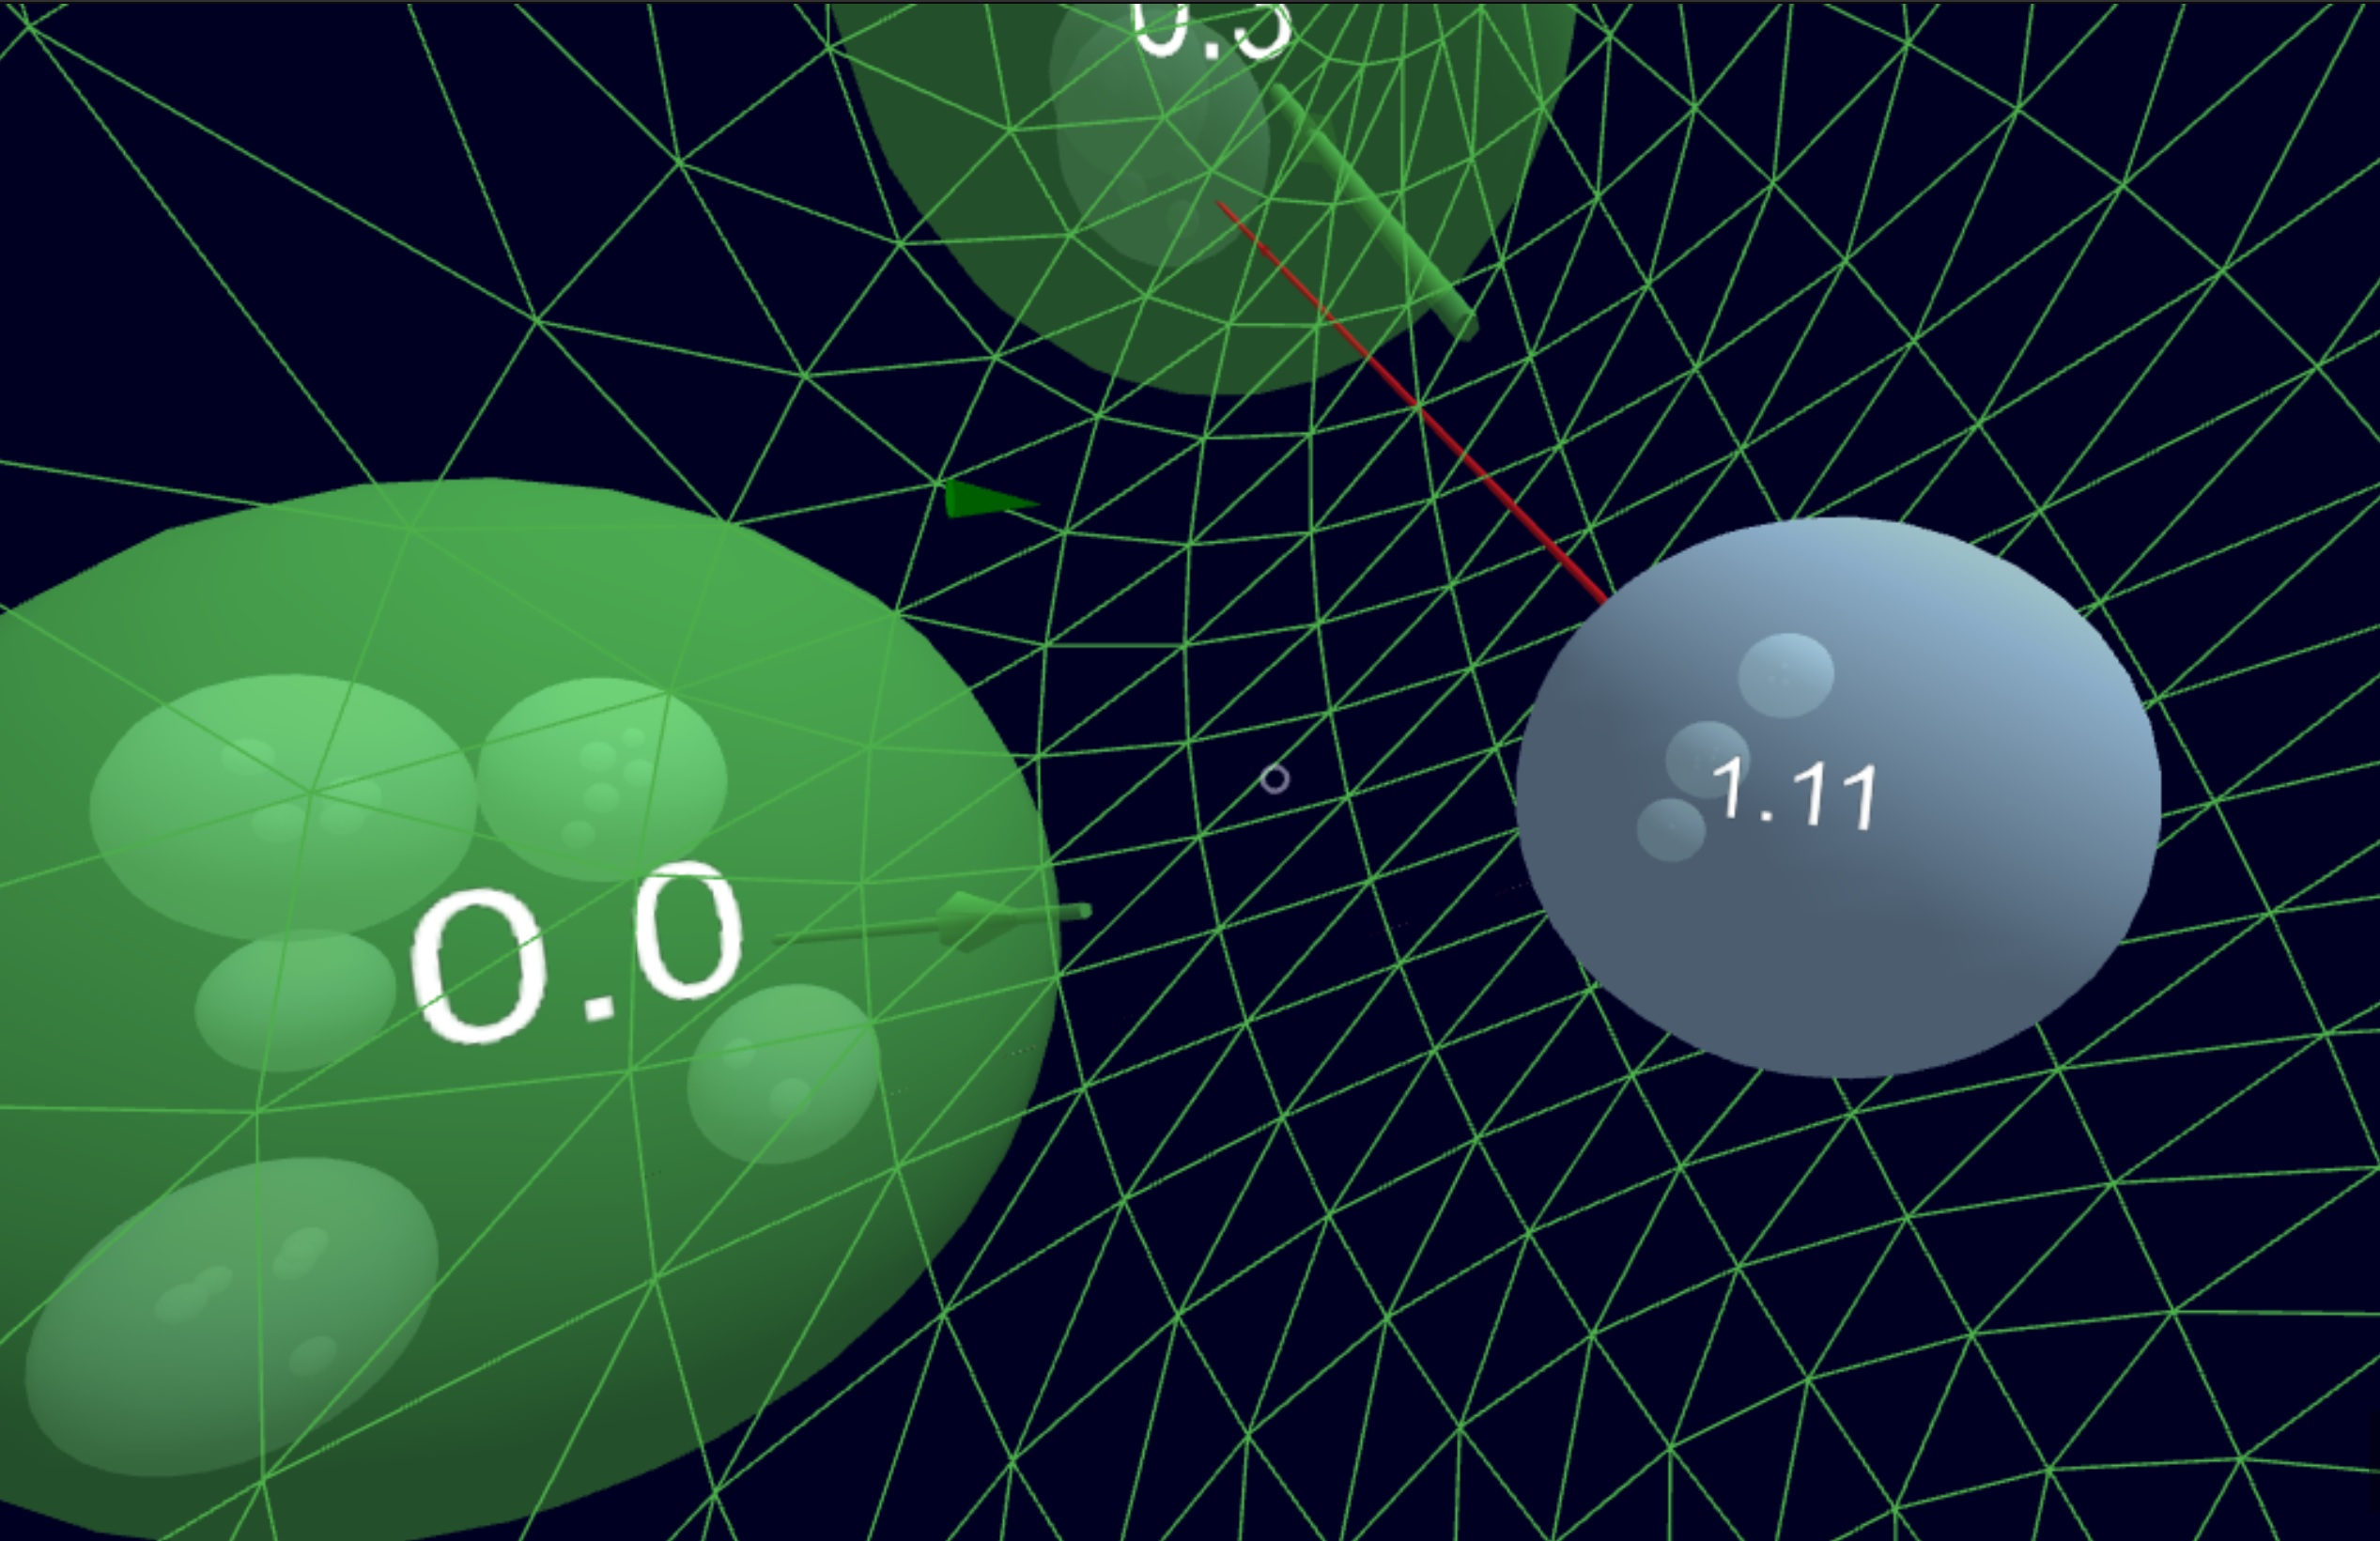
\includegraphics[width=1\textwidth]{graphics/screenshotNestingAndWireframe.jpg}
    \caption[Screenshot of the visualization.]{Detail perspective inside of node 0.2: To be able to tell the border of the nodes, the node is rendered as a wireframe when looking from the inside out.}
    \label{fig:ps_wireframe}
\end{figure}
The goal of the graph visualization was to choose appropriate visual encoding which allow us to reduce visual clutter and improve clarity while still displaying as much data as possible.
To represent the graph, we choose spheres for nodes, tubes as links and cones as arrow heads indicating the link direction.
With solid textures, the overview ability of the visualization would be poor since our layout approach uses nested layers. Therefore, the user could only see one layer of nodes at the same time. To circumvent that we render all nodes transparently. Then, the user is able to see the nested nodes inside their parent node (see Figure \ref{fig:ps_nestedLayout}). 
However, links inside other nodes are not visible because displaying many links would increase visual clutter and reduce overview. To deal with the large amount of links, we apply filter conditions, which are described in Section \ref{chap:ps-filterLinks}.
When the user is inside a node, the transparent sphere of the node is not rendered anymore. Instead of a solid transparent sphere, we render a wireframe (see Figure \ref{fig:ps_wireframe}). The improved spatial impression given by the virtual reality experience allows the user to better see the boundary of the wireframe than visible in the Figure. To further improve the assignability of nodes to their layers, each node and link of the same layer shares a predefined color.
For each node instance, a billboard text label is placed on the border of the node and always points towards the camera. For our artificially dataset the ID of the node is displayed, for a real dataset it would display the appropriated node and cluster names.

Our adapted sphere packing layout algorithm requires us to render nodes and links smaller for each nested sphere. To achieve that, we added a dynamically scaling factor that is applied for each rendering entity (node, link, text-label). 
In addition to the rendering algorithm, the force algorithms also uses that scaling factor to ensure a correct collision detection and sphere packing. 
This globally scaling factor is described by the following formula: 
\begin{equation}
    s_{ d } = \frac{1}{(d+1)^{(d+1)} \cdot s}
\end{equation}
Where $s_{ d }$ is the resulting scaling factor, $d$ is the depth of the current layer and $s$ is a global constant that allows us to balance the force algorithm according to the rendering objects. The resulting scaling factor is used, in combination with the number of child nodes, to calculate the size of the node: 
\begin{equation}
    r_{ d,i } = (r \cdot s_{ d }) + (\left\lvert N_{ d,i } \right\rvert \cdot rs)
\end{equation}
Where $d$ is the depth, i the node index at depth $d$, r is a base radius, $s_{ d }$ is the previous scaling factor, $\left\lvert N_{ d,i } \right\rvert$ is the set of child nodes of the node $i$ at depth $d$, and $rs$ is a global constant to balance the size of the node radius to the according force radius.

\section{Interaction}
\label{chap:solution-interaction}

\begin{figure}[b]
    \centering
    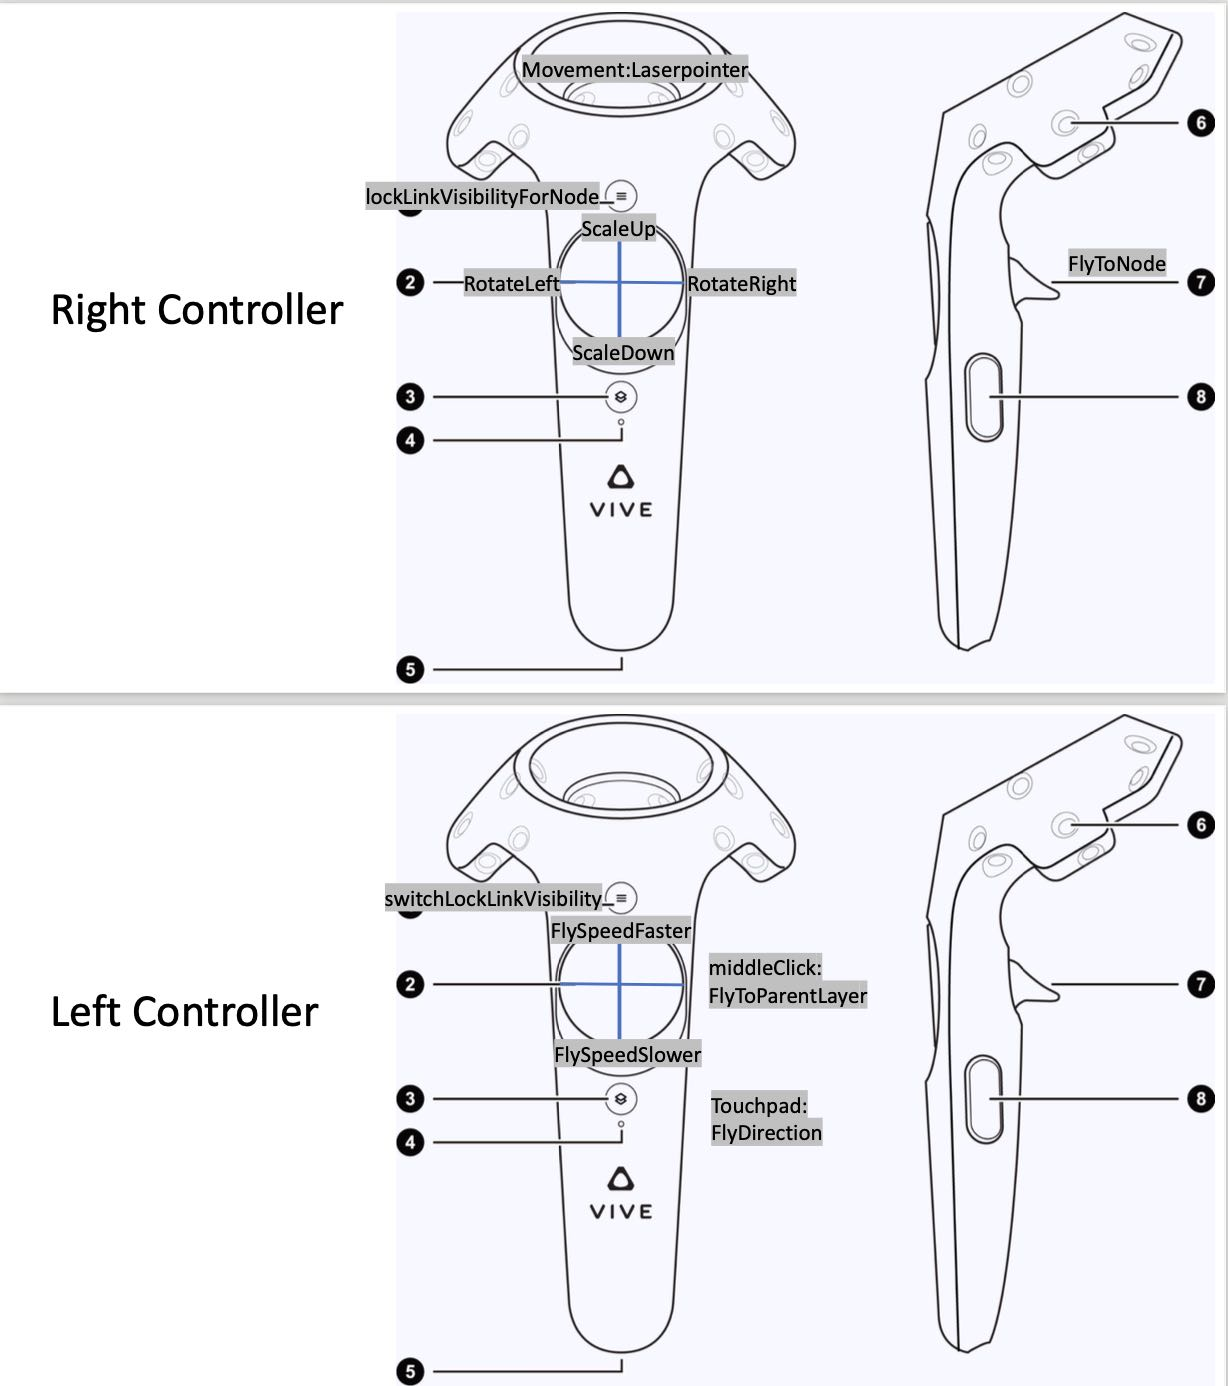
\includegraphics[width=1\textwidth]{graphics/controllerMapping.jpg}
    \caption[Our controller mapping for the interactive VR experience.]{Our controller mapping for the interactive VR experience. Depending on the clicking position on the touchpad, different actions can be called. The different clicking positions are marked in the image with different colors.} 
    \label{fig:controllerMapping} 
\end{figure}
For achieving \hyperref[req:R4]{R4}, we use the 6 DOF tracking of the headset and controllers from the HTC Vive. Therefore, we aimed to implement intuitive interaction techniques to allow teleportation navigation throughout the virtual scene (see Section \ref{chap:solution-navigation}). In addition, the user should be able  to switch the visibility filter between multiple groups of links (see Section \ref{chap:ps-filterLinks}).
What both interactions have in common is that the user has to select a specific node before these actions can be triggered. 
This concludes that our visualization needs a general way to support the selection of nodes which then can be used by various other methods we apply during the exploration process. 
In addition, we also stated in our requirements that we strive to use the tracking capabilities of VR to create intuitive interaction methods.
Therefore, all user interactions can only be provided by the native VR supported hardware, in particular from 6-DOF tracked controllers. 
To this end, we use the common concept of ray cast selection for selecting nodes in the virtual scene. Along the length of the right controller, a ray is cast through the scene. 
To better visualize the effect, we render a straight red line to imitate a virtual laser pointer (see Figure \ref{fig:screenshot_interaction}). 
The first intersected node is then used as the selected node for other methods like filtering or teleportation. The node label of the selected node is displayed in a Head-up-Display element centered in the lower part of the screen inside the headset (see Figure \ref{fig:screenshot_interaction}). 
In addition, the selected node and directly connected nodes are visually highlighted (see Figure \ref{fig:screenshot_interaction}). This allows the users to quickly see, which node they currently have selected and provides the context of the connected nodes.

\begin{figure}[h]
    \centering
    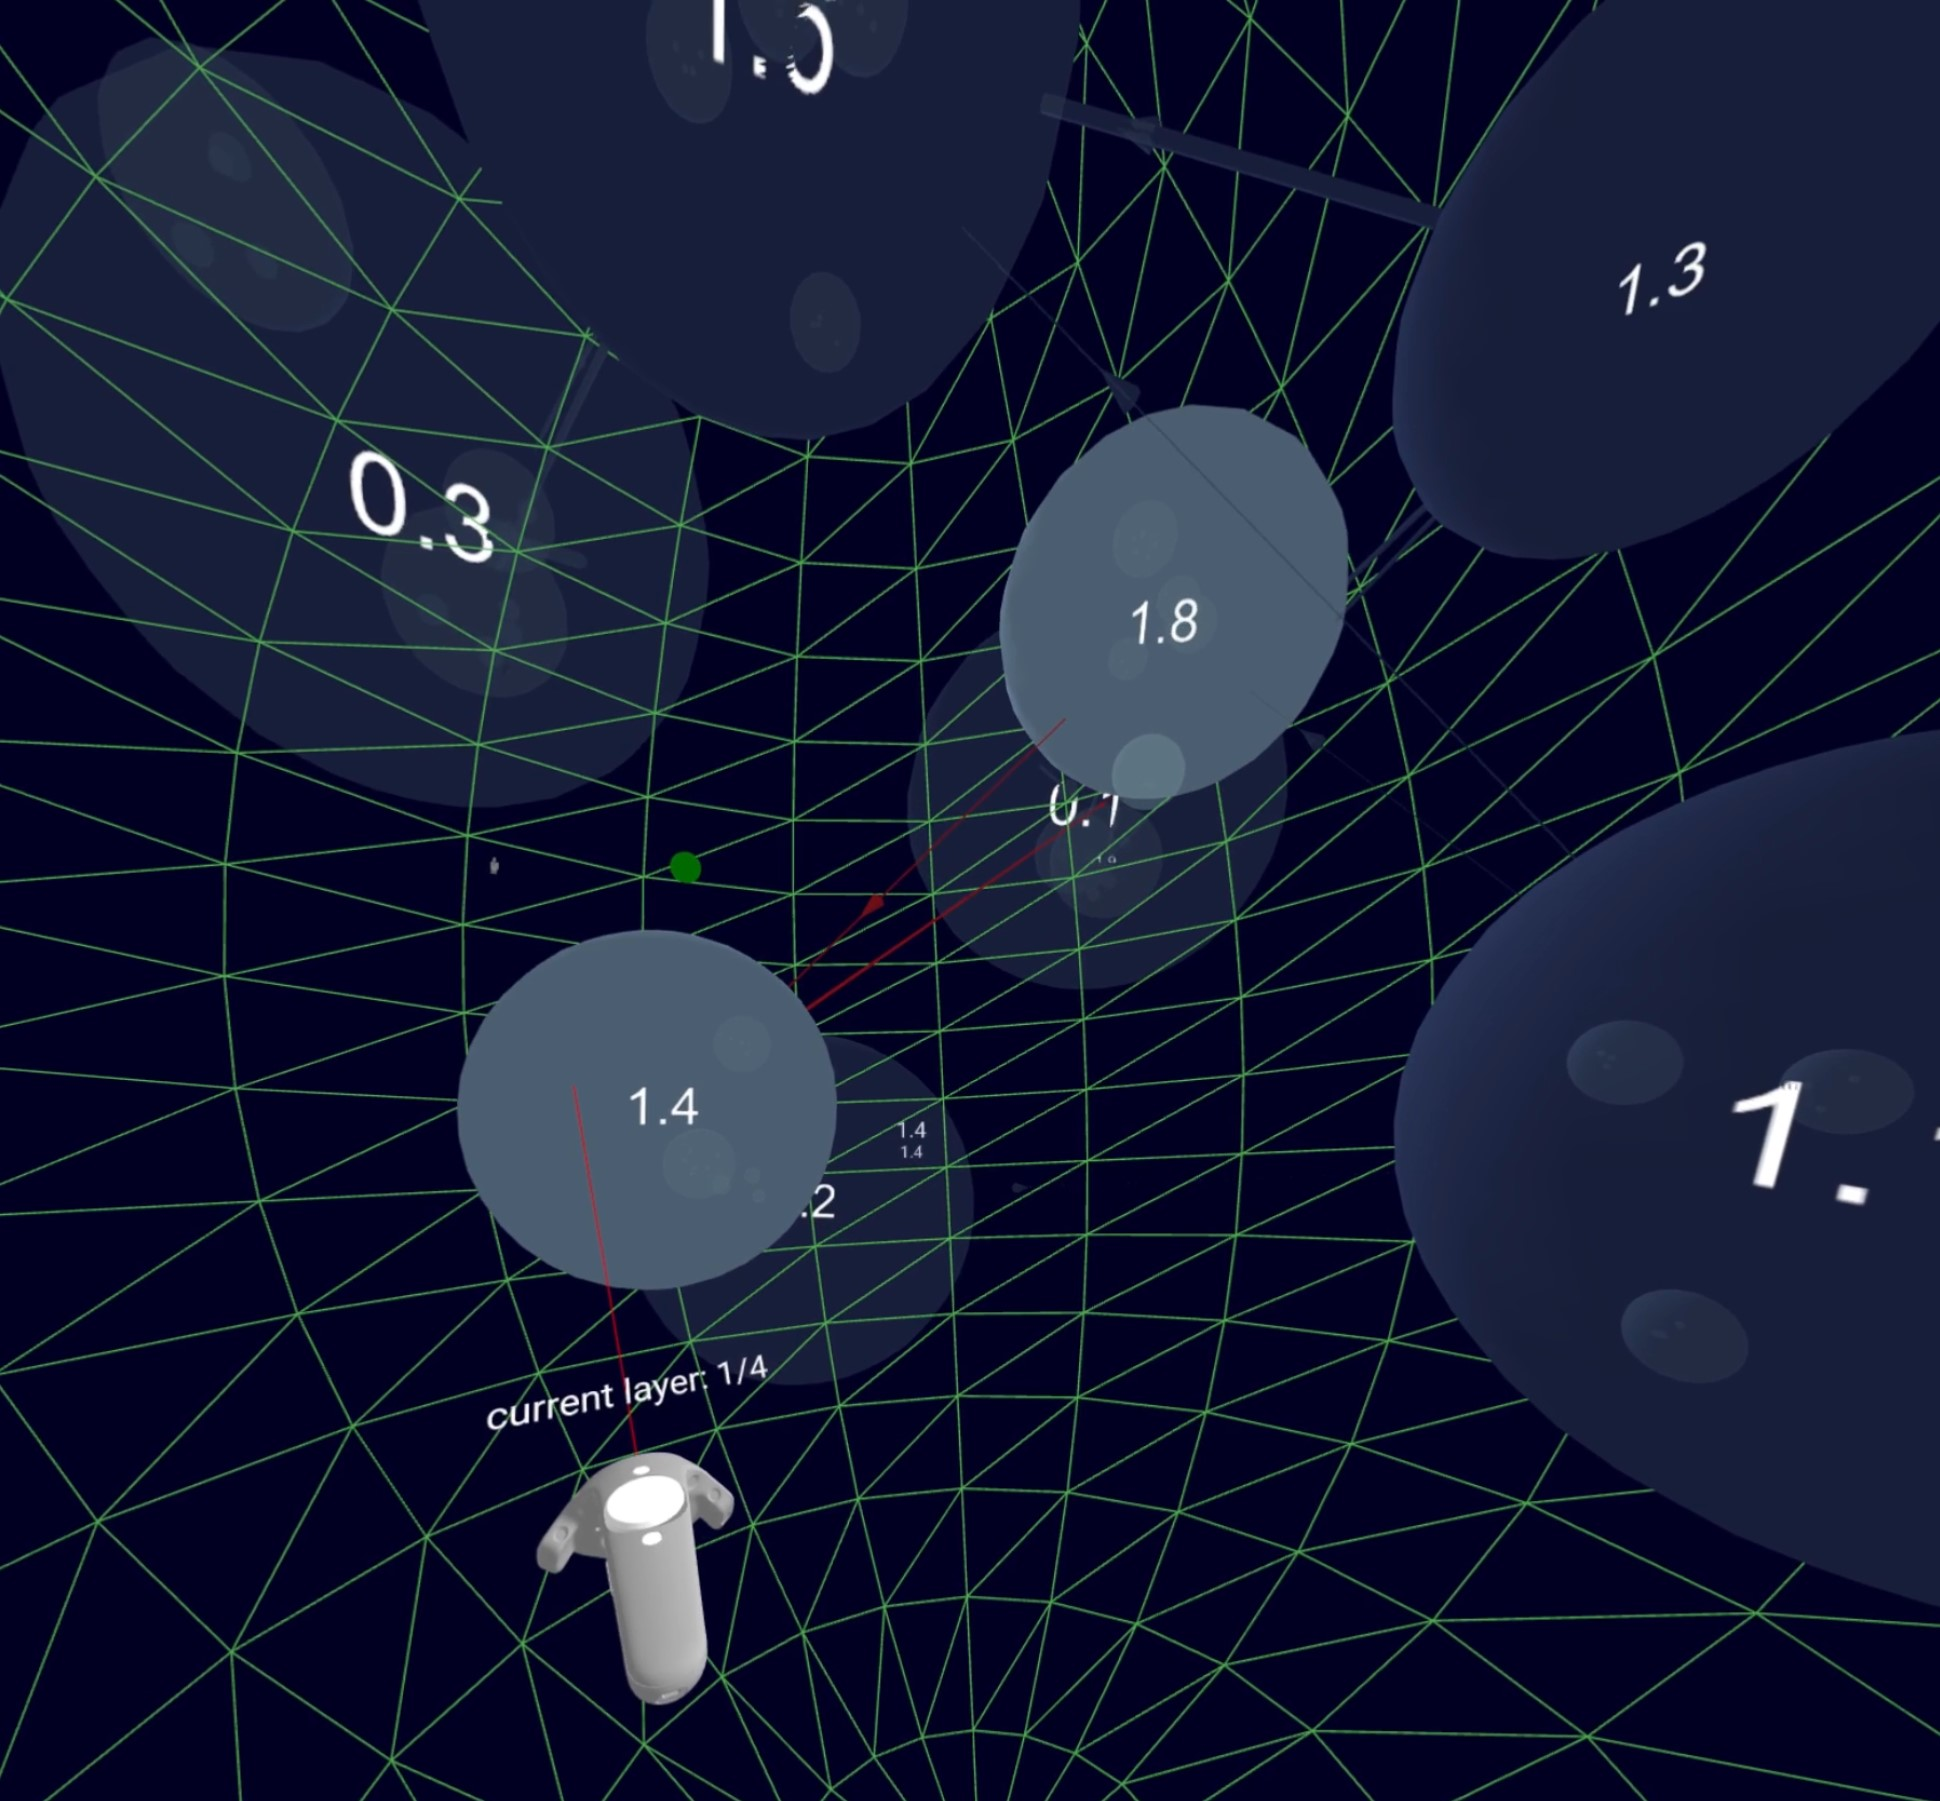
\includegraphics[width=1\textwidth]{graphics/screenShotFilteringNodes2.jpg}
    \caption[Screenshot during the selection of a node.]{Screenshot during the selection of a node: The user can see the virtual laser pointer as a red line. 
    In the lower part of the screen, the node label (1.4) of the pointed node is written (in this screenshot it is centered in the middle of the screenshot, because the field of view in the headset is different as in the screenshot).
    In addition, the selected node, as well as directly connected nodes, are highlighted in a brighter shading. For improved navigation, the layer where the user currently is located in is displayed as a text above the controller.} 
    \label{fig:screenshot_interaction} 
\end{figure}

Now that the users can select specific nodes in the scene, we also have to give them the opportunity to trigger certain actions. These actions include the teleportation navigation (see Section \ref{chap:solution-navigation}) and the link visibility filter (see Section \ref{chap:ps-filterLinks}). 
Other actions do not require the selection of a node, i.e., manual rotation, free flying with an adjustable flying speed, and teleportation to an upper layer (see Section \ref{chap:solution-navigation}), as well as manual scaling (see Section \ref{chap:ps-spatialReference}).\\
However, we have to assign each of these actions to a button on the controller (see Figure \ref{fig:controllerMapping}). In order to provide a smooth workflow, we extend the normal trackpad click by the position of clicking. 
This allows us to have 5 virtual buttons on the trackpad: top, bottom, left, right and center. The advantage of this method is that these virtual buttons can be used fluently while also interacting with the touch sensitive trackpad at the same time by one finger. 
Therefore, the users can control the free flying direction and speed with their left thumb, as well as triggering the teleportation to the upper hierarchical layer. The right controller acts as a virtual laser pointer. The two actions, which need a node selection beforehand, can be started by the menu button and trigger. 
On the right trackpad, the scaling and rotation can be controlled.

We optimized our application for the HTC Vive. Therefore, all described button mappings refer to the HTC Vive controllers. However, we only use simple buttons, trackpads and industry standard tracking methods. 
As other 6-DOF headsets usually provide the same or similar interaction possibilities, the interaction concept of our visualization can be applied to other headsets as well.

\subsection{Filtering Link Visibility}
\label{chap:ps-filterLinks}

\begin{figure}[p]
    \centering
    \begin{subfigure}{0.6\columnwidth}
        \centering
        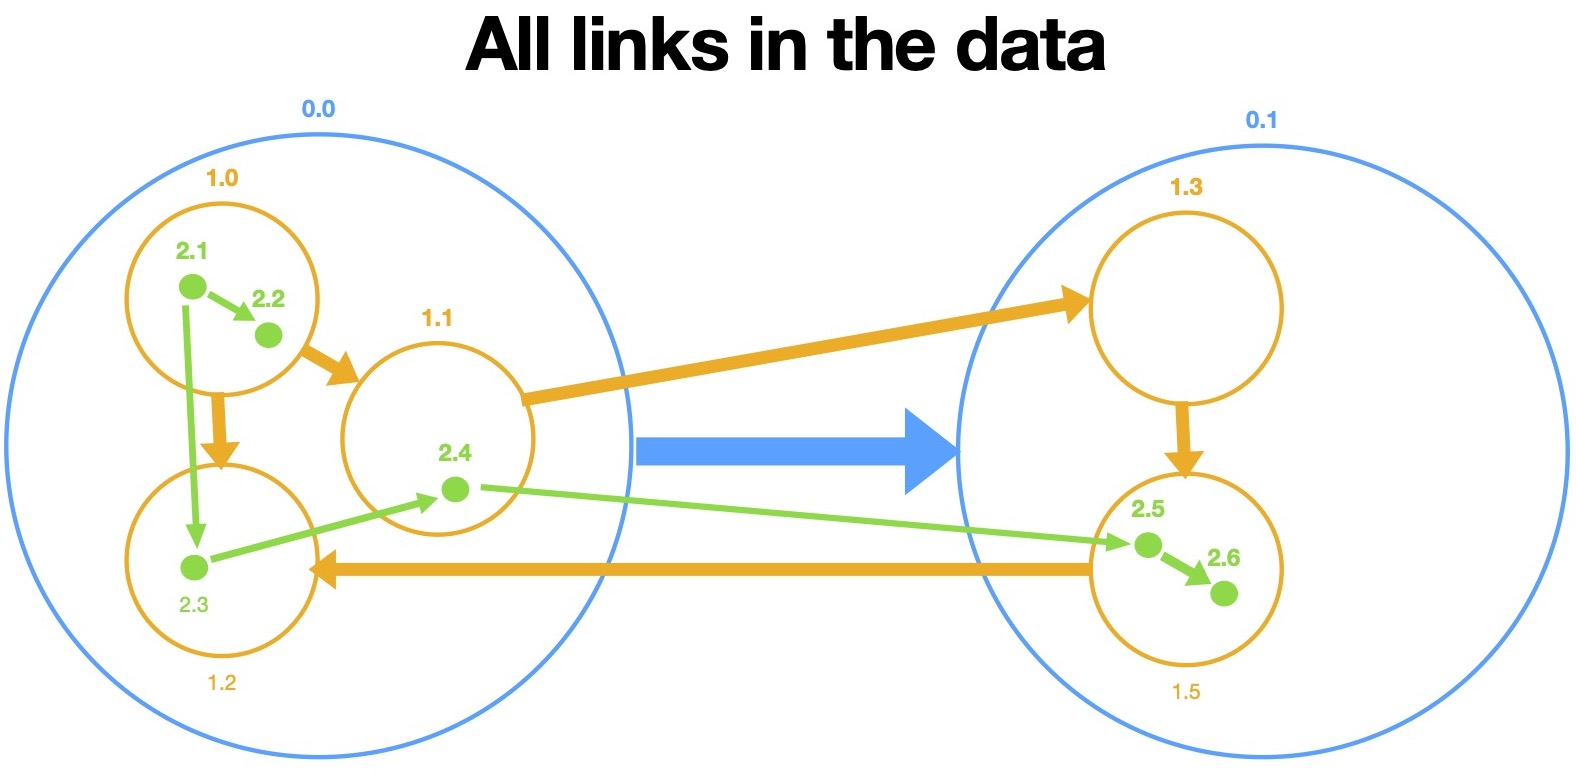
\includegraphics[width=\textwidth]{graphics/filterLinks/allLinks.jpg}
        \subcaption{All links represented in the data.}
        \label{fig:linkFilter-all}
    \end{subfigure}
    \begin{subfigure}{0.6\columnwidth}
        \centering
        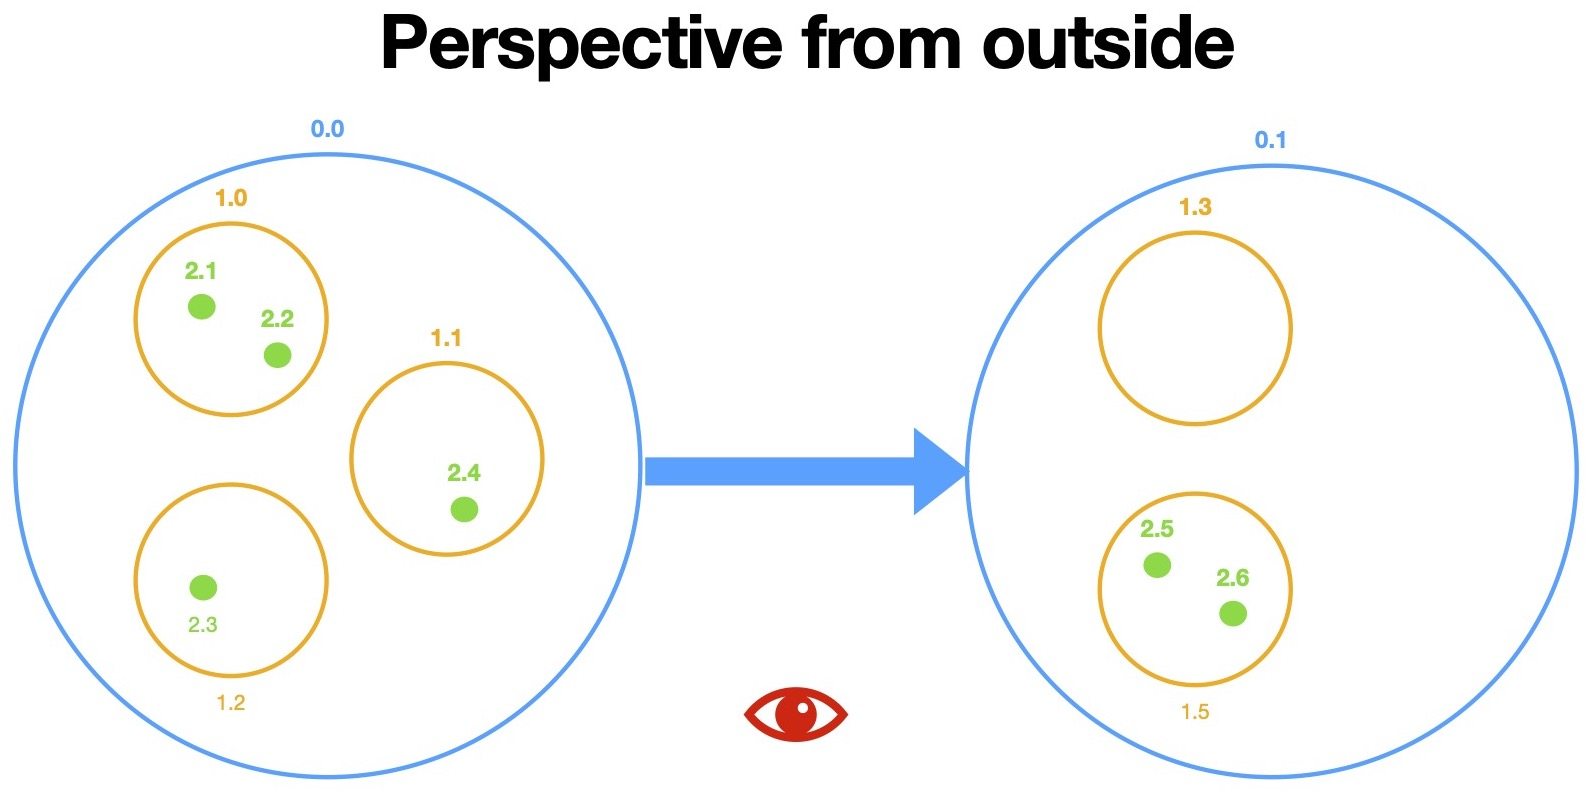
\includegraphics[width=\textwidth]{graphics/filterLinks/outside.jpg}
        \subcaption{Visible links when the user is outside every node.}
        \label{fig:linkFilter-outside}
    \end{subfigure}
    \begin{subfigure}{0.6\columnwidth}
        \centering
        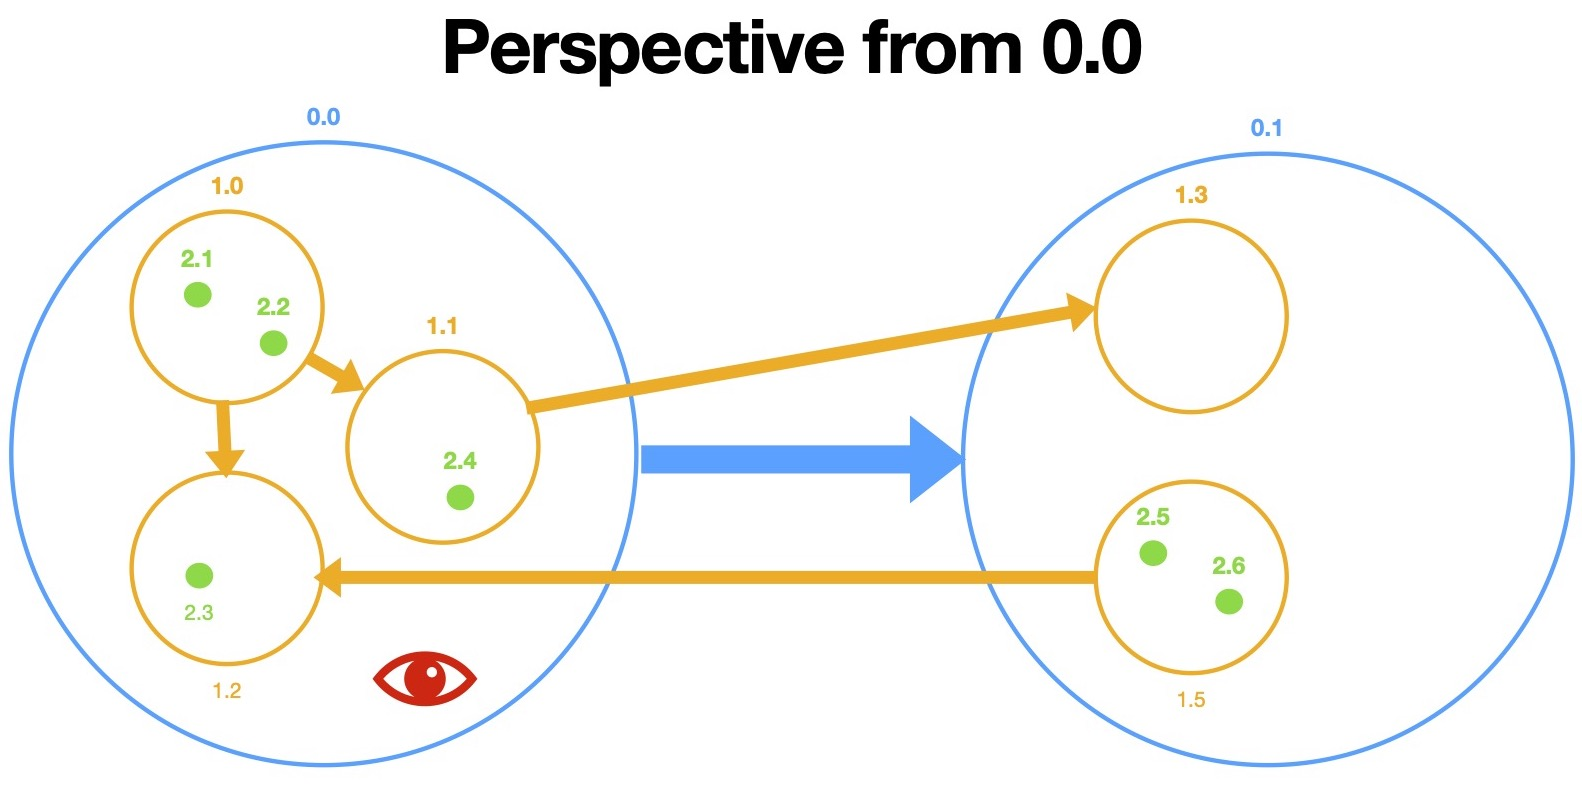
\includegraphics[width=\textwidth]{graphics/filterLinks/layer0.jpg}
        \subcaption{Visible links when the user is inside node 0.0 or when node 0.0 is selected by the laser pointer interaction.}
        \label{fig:linkFilter-layer1}
    \end{subfigure}
    \begin{subfigure}{0.6\columnwidth}
        \centering
        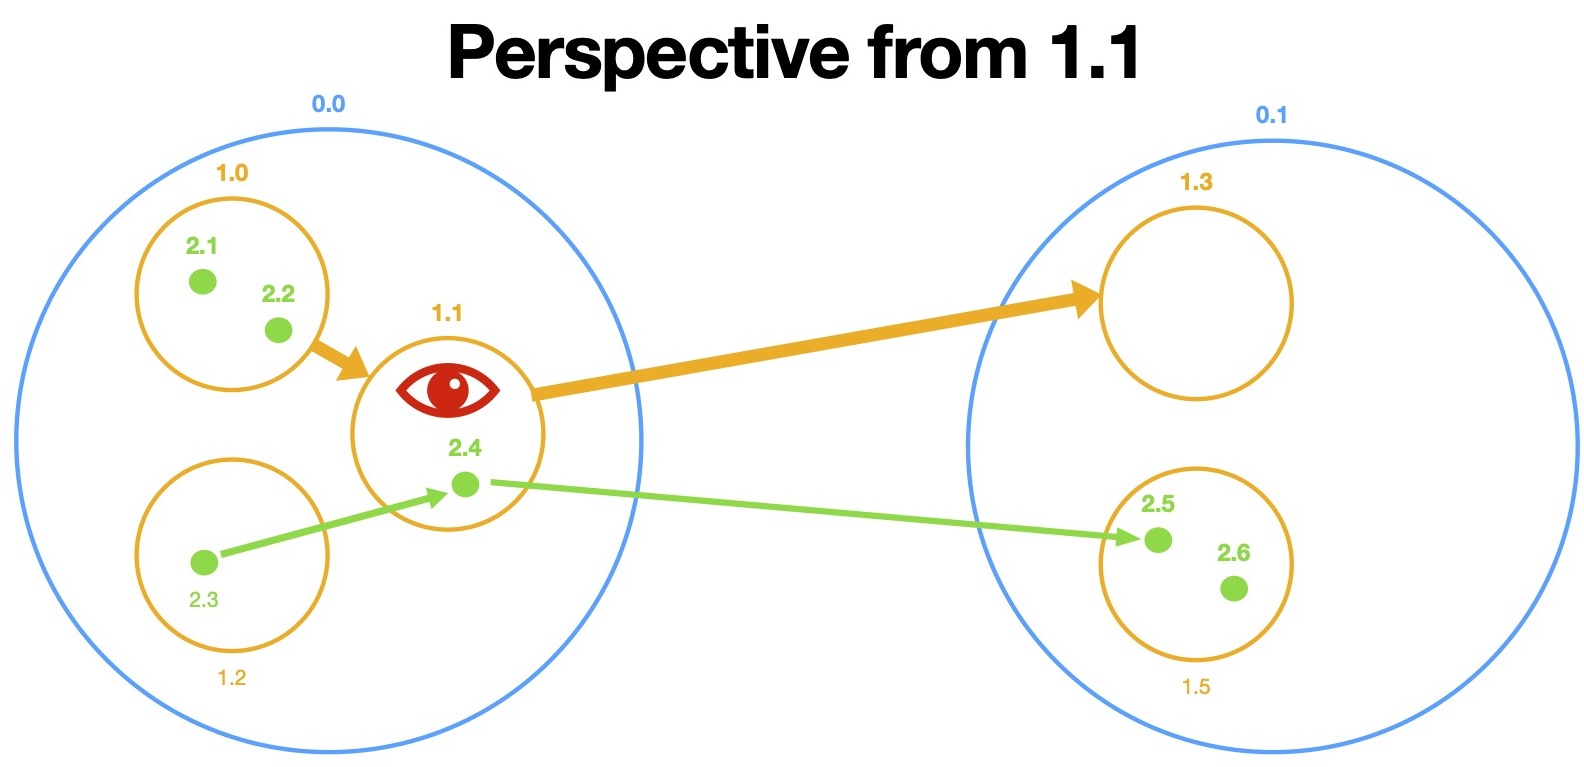
\includegraphics[width=\textwidth]{graphics/filterLinks/layer1.jpg}
        \subcaption{Visible links when the user is inside node 1.1 or when node 1.1 is selected it by the laser pointer interaction.}
        \label{fig:linkFilter-layer2}
    \end{subfigure}
    \caption{Our filtering technique visualized on a small example graph.} % Remove the [...] argument if the original caption should be used in the figure list.
  \end{figure}

To ensure the clarity of the visualization (see \hyperref[req:R6]{R6}) and display larger networks than 2D approaches (see \hyperref[req:R2]{R2}), we apply a filtering approach for links according to the requirements. 
The goal is to reduce visual clutter while providing as much information as possible. 
As a quick recap: Links in our visualization can exist between nodes within the same hierarchical parent node but also to nodes with a different parent node as long as the hierarchical depth is the same. Figure \ref{fig:linkFilter-all} shows a small example of all possible link combinations for three hierarchical layers.
Displaying all links at the same time would quickly lead to visual clutter where a meaningful exploration is not possible anymore. 
Therefore, we came up with our own filtering logic that decides which links are displayed and which are not. 
The filter uses a specific node. This can either be a directly selected node from the user (by the laser pointer interaction) or an indirectly selected node through the position of the user. A directly selected node always overrules the indirectly selected one. Our filter logic uses the following rules:

\begin{enumerate}
    \item If no node is selected and the user is not inside any node only the links from the top layer 0 are displayed (see Figure \ref{fig:linkFilter-outside}).
    \item All directly connected links to the selected node are displayed (currently our visualization only supports links between nodes with the same depth $d$).
    \item All links connected to direct child nodes from the selected node are displayed. Direct child means the depth of the child node is $d+1$. 
    \item All other links are not visible.
\end{enumerate}

As an example, Figure \ref{fig:linkFilter-layer1} shows a situation where node 0.0 is selected. Therefore, all links connecting direct neighbor-nodes of 0.0 and links to the child-nodes of 0.0 itself are displayed. However, links of deeper nested nodes, like 2.1, are not displayed. 
A different situation can be seen in Figure \ref{fig:linkFilter-layer2}: here only links from node 1.1 and 2.4 are visible but the links from node 1.2 and 0.0 are not visible anymore.
In an earlier version, we not only displayed the links of direct child nodes but instead links of all recursive child nodes. For example, in Figure \ref{fig:linkFilter-layer1}, the green links would also be visible. However, this quickly leads to visual clutter. Therefore, we kept the direct child approach.

In order to support an intuitive and flexible exploration workflow, the user also has the ability to lock a currently applied filter.
With the left menu button (see Figure \ref{fig:controllerMapping}), the state of the lock can be toggled. 
If the lock is active, the indirect selection of nodes by the position of the user is disabled. The lock is also automatically set active if a node is manually selected by the laser pointer. 
This allows the user to freely navigate around the visualization without constantly having to deal with changing link visibility. 
On freeing the lock, the indirect selection of nodes automatically kicks in again and selects the current node the user is positioned in.

\section{Navigation}
\label{chap:solution-navigation}
In order to fulfill \hyperref[req:R3]{R3}, we support a walkable room scale VR experience setup to navigate the virtual scene. As we stated in Section \ref{chap:rw-vrnavigation}, walking probably provides the best immersive and intuitive navigation method.
However, the graph will usually be larger than the user's available space. To this end, we also include other navigation methods.
To allow maximum of flexibility during the navigation, as required for \hyperref[req:R5]{R5}, we provide two navigation methods: animated teleporting for covering larger distances and free flying to perform small and precise position adjustments.

The user should be able to move to other distant parts of the graph without loosing orientation or being interrupted in the exploration flow. A common example is to jump to a connected node of another parent node. 
Therefore, we implemented an animated teleportation method. The user can select a node with the laser pointer and then press the right trigger to initiate the teleportation. The target position is the closest edge barely inside the node. This allows the user to get an overview of all nodes and links in that selected node.   
As with a simple teleportation over long distances, the user might lose the orientation. Therefore, we perform a short animation to the target position. The speed of the animation is adapted with an ease-in and ease-out transition.
Remember that, as soon as the user enters another node, the visibility of links changes, provided there is no active lock.
Instead of teleporting deeper into the hierarchical network, the user can also teleport to the parent hierarchical layer; in particular to the area barely outside the node the user is currently located in. This teleportation can be triggered by pressing the middle of the left trackpad.
All teleportation methods can be freely combined even during the animation, therefore allowing the user to fluently move around the graph. 
To further improve the overview, we display the current hierarchical layer as a text element floating over the right controller (see Figure \ref{fig:screenshot_interaction}). 

To perform small adjustments in position, especially when the user's free space is limited, the user can freely fly in the virtual scene. To control the direction, the left touch sensitive trackpad can be used. 
The forward direction is linked to the user's gaze direction, so the final fly direction is the combination of gaze direction and trackpad touch position. 
In addition, the fly speed is adjustable with a click on top or bottom of the trackpad.    
Similar to other VR applications, we also implemented rotation of the entire room scale space in the virtual scene. This allows the users to better position themselves in the real world. 
This is particularly useful with cable bound headsets because multiple rotations in the real world require the user to step over the cable. In other VR applications, movement is usually carried out with the left controller and rotation with the right, analogous to Gamepad controls in most games. Therefore, we mapped the rotation to the right trackpad by clicking either on the left or right corner.

\subsection{Challenge of Spatial Reference in VR}
\label{chap:ps-spatialReference}
In \hyperref[req:R7]{R7}, we stated that the visualization should reduce the problem of a multi scale scene.
The challenge is that nodes and links are getting exponentially smaller with each hierarchy step.
This introduces a new problem as after a few iterations, the nodes and links in the virtual scene are too small to recognize.
2D visualizations usually deal with that by adjusting the viewport of the visualization, e.g., zooming in and out. 
However, in the context of a 3D VR visualization, a simple 2D zooming approach is not possible due to the additional dimension. 
In a 3D non-VR visualization that problem can be mitigated by adjusting the movement speed. Therefore, distances seem similar in size for the inner nodes and navigation is also possible without overshooting the target position. 
In VR the situation is trickier due to the spatial impression through stereoscopic rendering. On a 2D projected image, like on a normal monoscopic computer screen, distances in the scene can only be estimated through movement. From a static image, the human eye is not able to recognize the distance or size of an object without any additional size reference. 
In the real world however, we constantly see objects with two eyes in a stereoscopic view, this enables the human mind to estimate distances without the need of any movement. VR works the same way by rendering the scene from two different perspectives each for one eye.  
This means that a simple trick of adjusting the movement speed is not working for our VR visualization.
That problem makes itself noticeable, for example, as layer 4 nodes in VR are the size of a needle where layer 0 nodes are the size of an entire house.
In addition to the perspective problem, changing the movement speed also does not work because movement in a 6-DOF VR headset is also always carried out by movement in the real world and obviously the physical movement speed can not be adjusted.

One solution to that problem is scaling the entire scene. Therefore, we implemented two techniques in our visualization:
\begin{itemize}
    \item Dynamically adjusting the fly speed while navigating in the graph. On entering a node, the speed slows down. When leaving, it speeds up again. 
    \item Dynamically scaling the entire scene. When teleporting to a node in a deeper hierarchy layer, an upscaling transition is started. On teleporting to the parent layer, a downscaling transition is started. 
\end{itemize}

\label{sec:scaling}
The challenge while scaling is that the user's relative position in comparison the to virtual scene must not change. Otherwise, the user will get distracted while exploring.
When applying a scaling matrix, the center of the scene (0,0,0) stays in the same position. All other points are moved during the scaling process. 
Therefore, we translate the target position of the animated teleport into the center of the scene, then scale up/down and afterwards translate the scene back.
In order to achieve a smooth user-friendly scaling, instead of scaling to the desired size once, we animate the scaling process. The duration of the animation has to be the exact time as the animated teleportation. 
Otherwise, the teleportation path will get distorted and result in a curve instead of a straight line.
The automated scaling process is described by the formula:
\begin{equation}
    S_{ p } = T_{ p } \cdot S_{ i } \cdot T_{ p }^{ -1 }
\end{equation}
Where $S_{ p }$ is the scaling matrix for the target flying teleport position $p$, $T_{ p }$ is the translation matrix from the position to the center, $T_{ p }^{ -1 }$ the reverse translation matrix and $S$ a usual 3D scaling matrix for a given scaling size $i$.

In addition, the scale can also be manually changed by the user at any time by pressing the upper or lower corner of the right trackpad. 
In \hyperref[req:R3]{R3}, we stated to support small and large room sizes.
However, the scale can not be optimized beforehand for a walking experience. The manual scaling gives the users the ability to adjust the scale to their available space and personal preference.
In the manual scaling process we have to distinguish between the rig and camera position. The reason for this is how camera movement in VR frameworks are handled (see Section \ref{sec:vrInteractions}).
The manual scaling process is described by the formula:

\begin{equation}
    S_{ p } = T_{ p_{ rig } } \cdot T_{ p_{ camera } } \cdot S \cdot T_{ p_{ camera } }^{ -1 } \cdot T_{ p_{ rig } }^{ -1 }
\end{equation}
Where $S_{ p }$ is the scaling matrix for the current user's position $p$, $T_{ p_{ rig } }$ is the translation matrix from the relative rig position to the center, $T_{ p_{ camera } }$ is the translation matrix from the relative camera position to the center, $T_{ rig }^{ -1 }$ and $T_{ camera }^{ -1 }$ the reverse translation matrices and $S$ a usual 3D scaling matrix for a given scaling size $i$.

\section{Exploration Flow}
\label{chap:ps-explorationFlow}
To provide an optimal exploration experience of the hierarchical network, we use the overview and detail concept of the visual information seeking mantra (see Section \ref{seeking mantra}) as stated in \hyperref[req:R6]{R6}. 
At the beginning of an exploration session, the user is in the overview perspective. The user is placed on a further position away from the center where a good overview of the entire graph is possible. In addition, rotation to the graph can be applied.
When the user decides to dive deeper into the network, a node can be selected via the ray cast controller interaction. This triggers the transition into the detail perspective. 
Here all navigation and interaction methods described in Sections \ref{chap:solution-interaction} and \ref{chap:solution-navigation}
are available. 
A core concept for the exploration in the detail perspective is the use of the VR room-scale navigation experience. As the user is able to tweak the scale of the scene to their liking, walking around the graph is possible for different room sizes. The goal is to improve the spatial impression of the graph, which results in a better clarity and understanding of the data.